\documentclass[a4paper]{article}

\usepackage[utf8]{inputenc}
\usepackage{listings}
\usepackage{hyperref}
\usepackage{tikz}
\usepackage{scalefnt}
\usepackage{microtype}

\parindent 8pt
\parskip 2pt

\lstset{tabsize=2, basicstyle=\small, breaklines=true, numbers=left, language=c++}

\title{libea 0.2 - A brief introduction}
\author{Sebastian Fedrau}
\date{February, 2015}

\begin{document}

\maketitle

\newpage

\section{Introduction}

\textsc{libea} is a template based library written in C++14. The purpose of this software is to provide an extensible and reliable framework for writing evolutionary algorithms.

\section{Building libea}

To build \textsc{libea} scons\footnote{\url{http://www.scons.org/}} is required. The library can be compiled and installed with the following commands:

\begin{lstlisting}[language=bash, numbers=none]
# scons libea
# sudo scons install
\end{lstlisting}

After the installation you may want to build the test suite. Please note that this step requires the CppUnit\footnote{\url{http://freedesktop.org/wiki/Software/cppunit/}} framework:

\begin{lstlisting}[language=bash, numbers=none]
# scons test-suite
\end{lstlisting}

If you want to generate the source code documentation please ensure Doxygen\footnote{\url{http://www.stack.nl/~dimitri/doxygen/}} is installed on your system and type in the following command:

\begin{lstlisting}[language=bash, numbers=none]
# scons doc
\end{lstlisting}

This documentation can be build with

\begin{lstlisting}[language=bash, numbers=none]
# scons pdf
\end{lstlisting}

If you want to uninstall libea type in

\begin{lstlisting}[language=bash, numbers=none]
# sudo scons install -c
\end{lstlisting}

\section{The framework}

\subsection{A quick overview}

In \textsc{libea} individuals are represented in \textit{sequences}. Theoretically any data type large enough to store the genotype of an individual is a valid sequence type. A group of sequences is called \textit{population}.

To modify a sequence or evaluate its fitness a corresponding \textit{genome base class} inherited from \textit{ea::AGenomeBase} is required. Figure~\ref{fig:overview} illustrates this concept.

\begin{figure}[h]
\caption{sequences and corresponding genome base class}
\label{fig:overview}
{\scalefont{0.6}
% Graphic for TeX using PGF
% Title: E:\git\libea\tex\img\overview.dia
% Creator: Dia v0.97.2
% CreationDate: Fri Nov 14 13:46:43 2014
% For: fedra001
% \usepackage{tikz}
% The following commands are not supported in PSTricks at present
% We define them conditionally, so when they are implemented,
% this pgf file will use them.
\ifx\du\undefined
  \newlength{\du}
\fi
\setlength{\du}{15\unitlength}
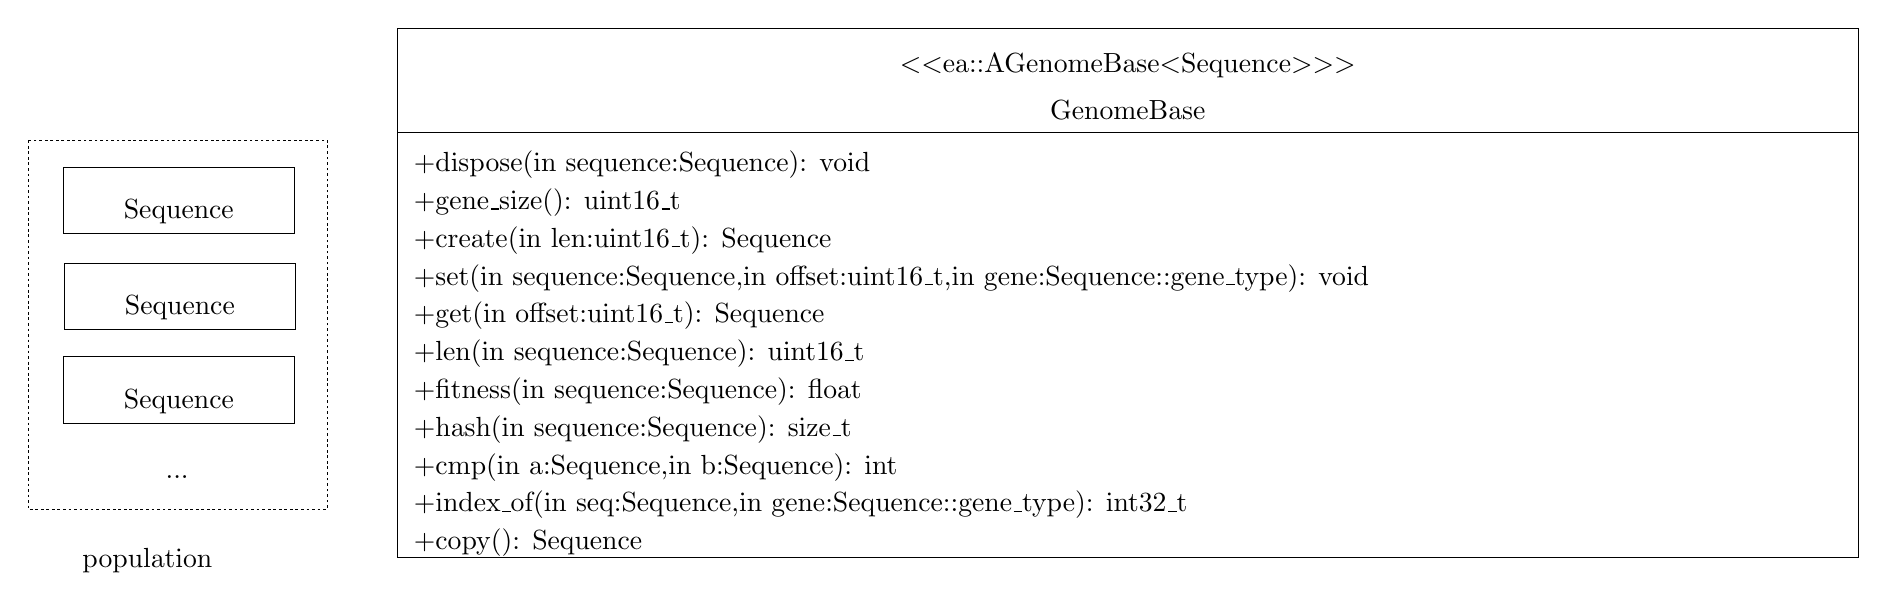
\begin{tikzpicture}[scale=0.6]
\pgftransformxscale{1.000000}
\pgftransformyscale{-1.000000}
\definecolor{dialinecolor}{rgb}{0.000000, 0.000000, 0.000000}
\pgfsetstrokecolor{dialinecolor}
\definecolor{dialinecolor}{rgb}{1.000000, 1.000000, 1.000000}
\pgfsetfillcolor{dialinecolor}
\pgfsetlinewidth{0.100000\du}
\pgfsetdash{{1.000000\du}{1.000000\du}}{0\du}
\pgfsetdash{{1.000000\du}{1.000000\du}}{0\du}
\pgfsetmiterjoin
\definecolor{dialinecolor}{rgb}{0.000000, 0.000000, 0.000000}
\pgfsetstrokecolor{dialinecolor}
\draw (18.942700\du,3.416490\du)--(18.942700\du,11.223911\du)--(25.285025\du,11.223911\du)--(25.285025\du,3.416490\du)--cycle;
\pgfsetlinewidth{0.100000\du}
\pgfsetdash{}{0pt}
\definecolor{dialinecolor}{rgb}{1.000000, 1.000000, 1.000000}
\pgfsetfillcolor{dialinecolor}
\fill (19.694000\du,3.977370\du)--(19.694000\du,5.377370\du)--(24.584000\du,5.377370\du)--(24.584000\du,3.977370\du)--cycle;
\definecolor{dialinecolor}{rgb}{0.000000, 0.000000, 0.000000}
\pgfsetstrokecolor{dialinecolor}
\draw (19.694000\du,3.977370\du)--(19.694000\du,5.377370\du)--(24.584000\du,5.377370\du)--(24.584000\du,3.977370\du)--cycle;
% setfont left to latex
\definecolor{dialinecolor}{rgb}{0.000000, 0.000000, 0.000000}
\pgfsetstrokecolor{dialinecolor}
\node at (22.139000\du,4.927370\du){Sequence};
\pgfsetlinewidth{0.100000\du}
\pgfsetdash{}{0pt}
\definecolor{dialinecolor}{rgb}{1.000000, 1.000000, 1.000000}
\pgfsetfillcolor{dialinecolor}
\fill (19.715600\du,6.007280\du)--(19.715600\du,7.407280\du)--(24.605600\du,7.407280\du)--(24.605600\du,6.007280\du)--cycle;
\definecolor{dialinecolor}{rgb}{0.000000, 0.000000, 0.000000}
\pgfsetstrokecolor{dialinecolor}
\draw (19.715600\du,6.007280\du)--(19.715600\du,7.407280\du)--(24.605600\du,7.407280\du)--(24.605600\du,6.007280\du)--cycle;
% setfont left to latex
\definecolor{dialinecolor}{rgb}{0.000000, 0.000000, 0.000000}
\pgfsetstrokecolor{dialinecolor}
\node at (22.160600\du,6.957280\du){Sequence};
\pgfsetlinewidth{0.100000\du}
\pgfsetdash{}{0pt}
\definecolor{dialinecolor}{rgb}{1.000000, 1.000000, 1.000000}
\pgfsetfillcolor{dialinecolor}
\fill (19.696300\du,7.992870\du)--(19.696300\du,9.392870\du)--(24.586300\du,9.392870\du)--(24.586300\du,7.992870\du)--cycle;
\definecolor{dialinecolor}{rgb}{0.000000, 0.000000, 0.000000}
\pgfsetstrokecolor{dialinecolor}
\draw (19.696300\du,7.992870\du)--(19.696300\du,9.392870\du)--(24.586300\du,9.392870\du)--(24.586300\du,7.992870\du)--cycle;
% setfont left to latex
\definecolor{dialinecolor}{rgb}{0.000000, 0.000000, 0.000000}
\pgfsetstrokecolor{dialinecolor}
\node at (22.141300\du,8.942870\du){Sequence};
% setfont left to latex
\definecolor{dialinecolor}{rgb}{0.000000, 0.000000, 0.000000}
\pgfsetstrokecolor{dialinecolor}
\node[anchor=west] at (21.660800\du,10.549200\du){...};
% setfont left to latex
\definecolor{dialinecolor}{rgb}{0.000000, 0.000000, 0.000000}
\pgfsetstrokecolor{dialinecolor}
\node[anchor=west] at (19.900600\du,12.303500\du){population};
\pgfsetlinewidth{0.100000\du}
\pgfsetdash{}{0pt}
\definecolor{dialinecolor}{rgb}{1.000000, 1.000000, 1.000000}
\pgfsetfillcolor{dialinecolor}
\fill (26.766600\du,1.034775\du)--(26.766600\du,3.234775\du)--(57.681600\du,3.234775\du)--(57.681600\du,1.034775\du)--cycle;
\definecolor{dialinecolor}{rgb}{0.000000, 0.000000, 0.000000}
\pgfsetstrokecolor{dialinecolor}
\draw (26.766600\du,1.034775\du)--(26.766600\du,3.234775\du)--(57.681600\du,3.234775\du)--(57.681600\du,1.034775\du)--cycle;
% setfont left to latex
\definecolor{dialinecolor}{rgb}{0.000000, 0.000000, 0.000000}
\pgfsetstrokecolor{dialinecolor}
\node at (42.224100\du,1.834775\du){\textless\textless ea::AGenomeBase\textless Sequence\textgreater\textgreater\textgreater};
% setfont left to latex
\definecolor{dialinecolor}{rgb}{0.000000, 0.000000, 0.000000}
\pgfsetstrokecolor{dialinecolor}
\node at (42.224100\du,2.784775\du){GenomeBase};
\definecolor{dialinecolor}{rgb}{1.000000, 1.000000, 1.000000}
\pgfsetfillcolor{dialinecolor}
\fill (26.766600\du,3.234775\du)--(26.766600\du,12.234775\du)--(57.681600\du,12.234775\du)--(57.681600\du,3.234775\du)--cycle;
\definecolor{dialinecolor}{rgb}{0.000000, 0.000000, 0.000000}
\pgfsetstrokecolor{dialinecolor}
\draw (26.766600\du,3.234775\du)--(26.766600\du,12.234775\du)--(57.681600\du,12.234775\du)--(57.681600\du,3.234775\du)--cycle;
% setfont left to latex
\definecolor{dialinecolor}{rgb}{0.000000, 0.000000, 0.000000}
\pgfsetstrokecolor{dialinecolor}
\node[anchor=west] at (26.916600\du,3.934775\du){+dispose(in sequence:Sequence): void};
% setfont left to latex
\definecolor{dialinecolor}{rgb}{0.000000, 0.000000, 0.000000}
\pgfsetstrokecolor{dialinecolor}
\node[anchor=west] at (26.916600\du,4.734775\du){+gene\_size(): uint16\_t};
% setfont left to latex
\definecolor{dialinecolor}{rgb}{0.000000, 0.000000, 0.000000}
\pgfsetstrokecolor{dialinecolor}
\node[anchor=west] at (26.916600\du,5.534775\du){+create(in len:uint16\_t): Sequence};
% setfont left to latex
\definecolor{dialinecolor}{rgb}{0.000000, 0.000000, 0.000000}
\pgfsetstrokecolor{dialinecolor}
\node[anchor=west] at (26.916600\du,6.334775\du){+set(in sequence:Sequence,in offset:uint16\_t,in gene:Sequence::gene\_type): void};
% setfont left to latex
\definecolor{dialinecolor}{rgb}{0.000000, 0.000000, 0.000000}
\pgfsetstrokecolor{dialinecolor}
\node[anchor=west] at (26.916600\du,7.134775\du){+get(in offset:uint16\_t): Sequence};
% setfont left to latex
\definecolor{dialinecolor}{rgb}{0.000000, 0.000000, 0.000000}
\pgfsetstrokecolor{dialinecolor}
\node[anchor=west] at (26.916600\du,7.934775\du){+len(in sequence:Sequence): uint16\_t};
% setfont left to latex
\definecolor{dialinecolor}{rgb}{0.000000, 0.000000, 0.000000}
\pgfsetstrokecolor{dialinecolor}
\node[anchor=west] at (26.916600\du,8.734775\du){+fitness(in sequence:Sequence): float};
% setfont left to latex
\definecolor{dialinecolor}{rgb}{0.000000, 0.000000, 0.000000}
\pgfsetstrokecolor{dialinecolor}
\node[anchor=west] at (26.916600\du,9.534775\du){+hash(in sequence:Sequence): size\_t};
% setfont left to latex
\definecolor{dialinecolor}{rgb}{0.000000, 0.000000, 0.000000}
\pgfsetstrokecolor{dialinecolor}
\node[anchor=west] at (26.916600\du,10.334775\du){+cmp(in a:Sequence,in b:Sequence): int};
% setfont left to latex
\definecolor{dialinecolor}{rgb}{0.000000, 0.000000, 0.000000}
\pgfsetstrokecolor{dialinecolor}
\node[anchor=west] at (26.916600\du,11.134775\du){+index\_of(in seq:Sequence,in gene:Sequence::gene\_type): int32\_t};
% setfont left to latex
\definecolor{dialinecolor}{rgb}{0.000000, 0.000000, 0.000000}
\pgfsetstrokecolor{dialinecolor}
\node[anchor=west] at (26.916600\du,11.934775\du){+copy(): Sequence};
\end{tikzpicture}

}
\end{figure}

\textsc{libea} offers the genome base class templates \textit{ea::PGenomeBase} and \textit{ea::CPGenomeBase} with the corresponding sequence types \textit{ea::Sequence} and \textit{ea::CSequence}. Any data type with a valid copy constructor is a supported gene type. There are already type aliases for many primitive data types available in \textsc{libea} (see table~\ref{tab:genome-base-classes-and-sequences}).

\begin{table}
\caption{genome base classes and corresponding sequence types offered by \textsc{libea}}
\label{tab:genome-base-classes-and-sequences}
\begin{tabular}{|l|l|l|}
\hline
\textsc{genome base class} & \textsc{corresponding sequence type} & \textsc{gene type} \\
\hline
ea::PGenomeBase\textless T\textgreater & ea::Sequence\textless T\textgreater & T \\
ea::Int32PenomeBase & ea::Sequence\textless int32\_t\textgreater & int32\_t \\
ea::UInt32PGenomeBase & ea::Sequence\textless uint32\_t\textgreater & uint32\_t \\
ea::BinaryPGenomeBase & ea::Sequence\textless bool\textgreater & bool \\
ea::DoublePGenomeBase & ea::Sequence\textless double\textgreater & double \\
ea::StringPGenomeBase & ea::Sequence\textless std::string\textgreater & std::string \\
\hline
ea::CPGenomeBase\textless T\textgreater & ea::CSequence\textless T\textgreater & T \\
ea::Int32CPenomeBase & ea::CSequence\textless int32\_t\textgreater & int32\_t \\
ea::UInt32CPGenomeBase & ea::CSequence\textless uint32\_t\textgreater & uint32\_t \\
ea::BinaryCPGenomeBase & ea::CSequence\textless bool\textgreater & bool \\
ea::DoubleCPGenomeBase & ea::CSequence\textless double\textgreater & double \\
ea::StringCPGenomeBase & ea::CSequence\textless std::string\textgreater & std::string \\
\hline
\end{tabular}
\end{table}

The two offered base class templates are optimized for different use-cases. As shown in listing~\ref{lst:sequence} the \textit{ea::Sequence} structure has only two fields which are used to store the length of a sequence and its genes. Hence this kind of sequence is preferable if the application's memory footprint is critical.

In comparison the \textit{ea::CSequence} structure has three additional fields. They are used to cache the evaluated fitness value and the hash of an individual (see listing~\ref{lst:csequence}). In general this sequence type is a better choice because the performance benefit might out weight the drawback of memory consumption.

The fields of both structures should \textbf{never be accessed directly}. \textsc{libea} provides the functions \textit{ea::sequence\_len()} and \textit{ea::sequence\_get()} for reading genes from a sequence.

\begin{lstlisting}[caption=Sequence template declaration, label=lst:sequence]
template<typename TGene>
struct Sequence
{
	/*! Datatype of stored genes. */
	typedef TGene gene_type;

	/*! Number of stored genes. */
	uint16_t len;
	/*! Dynamic array holding genes. */
	TGene* genes;
};
\end{lstlisting}

\begin{lstlisting}[caption=CSequence template declaration, label=lst:csequence]
template<typename TGene>
struct CSequence : Sequence<TGene>
{
	/*! Flags. */
	uint8_t flags;
	/*! Cached fitness value. */
	float fitness;
	/*! Cached hash value. */
	size_t hash;
};
\end{lstlisting}

\subsection{Core features}

\subsection{Working with sequences}

Listing~\ref{lst:core-functions} demonstrates some basic functions of \textsc{libea}. An individual represented in a sequence of integers is created (ll. 44-50) and copied (l. 62). The sequences are compared before and after modifying the second individual (ll. 67-75).

To access the genes and evaluate the fitness a genome base class is declared (l. 22). The template parameters specify the gene type and fitness function (ll. 5-19).

\begin{lstinputlisting}[caption=core functions,label=lst:core-functions]{examples/00-core-functions.cpp}
\end{lstinputlisting}

\subsection{Factories \& output adapters}

\textsc{libea} offers the \textit{ea::AFactory} base class as an option to create populations. Listing~\ref{lst:factory} shows how to create sequences of ten random integers using a custom factory (ll. 30-51). The values are generated with a random number generator (ll. 35-46).

The individuals are written to an \textit{ea::OutputAdapter} (ll. 74-77). At the current stage \textsc{libea} only provides an adapter for STL containers like \textit{std::vector}, but new adapters can be added easily by implementing the \textit{ea::IOutputAdapter} interface. To create an adapter use the \textit{ea::make\_output\_adapter()} function.

\begin{lstinputlisting}[caption=custom factory,label=lst:factory]{examples/01-factory.cpp}
\end{lstinputlisting}

\subsection{Selection operators}

Selection operators have to implement the \textit{ea::IIndexSelection} interface (see listing~\ref{lst:iindexselection}). Instead of copying the selected genomes to an \textit{ea::OutputAdapter} only the indexes are written. Access to the parent individuals is given through an adapter implementing the \textit{ea::IInputAdapter} interface. Input adapters can be created for all STL containers providing random access iterators with the \textit{ea::make\_input\_adapter()} function.

\begin{lstlisting}[caption=IIndexSelection,label=lst:iindexselection]
template<typename TGenomeBase>
class IIndexSelection
{
	public:
		typedef typename TGenomeBase::sequence_type sequence_type;

		~IIndexSelection() {}

		virtual void select(IInputAdapter<sequence_type>& input, const uint32_t count, IOutputAdapter<uint32_t>& output) = 0;
};
\end{lstlisting}

Listing~\ref{lst:selection-example} creates a population with ten random sequences (ll. 43-58). Then five individuals are selected using the tournament selection operator (ll. 72-82).

\begin{lstinputlisting}[caption=selection operators,label=lst:selection-example]{examples/02-selection.cpp}
\end{lstinputlisting}

\subsection{Crossover operators}

Crossover operators are inherited from \textit{ea::ACrossover} and have to override the \textit{crossover()} method (see listing~\ref{lst:acrossover}). 

\begin{lstlisting}[caption=ACrossover,label=lst:acrossover]
template<typename TGenomeBase>
class ACrossover
{
	public:
		typedef typename TGenomeBase::sequence_type sequence_type;

		~ACrossover() {}

		virtual uint32_t crossover(const sequence_type& a, const sequence_type& b, IOutputAdapter<sequence_type>& output) = 0;
};
\end{lstlisting}

Crossover operators create at least one child sequence from two parent individuals. The \textit{crossover()} method returns the number of child sequences written to the given output adapter. Listing~\ref{lst:crossover-example} shows an example.

In the example two parent individuals are created (ll. 41-42). Then two children are generated using a cycle crossover operator (ll. 51-55).

\begin{lstinputlisting}[caption=crossover operators,label=lst:crossover-example]{examples/03-crossover.cpp}
\end{lstinputlisting}

\subsection{Mutation operators}

Mutation operators are inherited from \textit{ea::AMutation} and have to override the \textit{create\_child()} method (see listing~\ref{lst:amutation}). 

\begin{lstlisting}[caption=AMutation,label=lst:amutation]
template<class TGenomeBase>
class AMutation
{
	public:
		typedef typename TGenomeBase::sequence_type sequence_type;

		virtual ~AMutation() {};

		virtual void mutate(sequence_type& sequence) = 0;

		sequence_type create_child(const sequence_type& sequence)
		{
			static TGenomeBase base;

			sequence_type m = base.copy(sequence);
			mutate(m);

			return m;
		}
};
\end{lstlisting}

In listing~\ref{lst:mutation-example} a parent individual is created (ll. 43-48) and mutated in-place (l. 55). Afterwards an inverted child sequence is generated (ll. 59-61).

\begin{lstinputlisting}[caption=mutation operators,label=lst:mutation-example]{examples/04-mutation.cpp}
\end{lstinputlisting}

\subsection{Processing operator pipelines}

The \textit{ea::Pipeline} namespace provides a framework to connect and process multiple genetic operators.

\textsc{libea} processes operators by connecting elements to a pipeline. Pipeline elements read sequences from a source and write the processed data to a sink. Each element has to implement the \textit{ea::Pipeline::IElelement} interface. \textsc{libea} offers a corresponding pipeline element for all operator types.

A functor implementing the \textit{ea::Pipeline::ITerminator} is executed after the last pipeline element has been processed to decide if the process should be repeated (see figure~\ref{fig:pipeline}).

\begin{figure}[h]
\caption{connecting pipeline elements}
\label{fig:pipeline}
{
% Graphic for TeX using PGF
% Title: E:\git\libea\tex\img\pipeline.dia
% Creator: Dia v0.97.2
% CreationDate: Mon Feb 02 17:23:50 2015
% For: sebastian.fedrau
% \usepackage{tikz}
% The following commands are not supported in PSTricks at present
% We define them conditionally, so when they are implemented,
% this pgf file will use them.
\ifx\du\undefined
  \newlength{\du}
\fi
\setlength{\du}{15\unitlength}
\begin{tikzpicture}
\pgftransformxscale{1.000000}
\pgftransformyscale{-1.000000}
\definecolor{dialinecolor}{rgb}{0.000000, 0.000000, 0.000000}
\pgfsetstrokecolor{dialinecolor}
\definecolor{dialinecolor}{rgb}{1.000000, 1.000000, 1.000000}
\pgfsetfillcolor{dialinecolor}
\pgfsetlinewidth{0.100000\du}
\pgfsetdash{}{0pt}
\pgfsetdash{}{0pt}
\pgfsetmiterjoin
\definecolor{dialinecolor}{rgb}{0.000000, 0.000000, 0.000000}
\pgfsetstrokecolor{dialinecolor}
\draw (7.900000\du,0.188656\du)--(7.900000\du,23.138656\du)--(35.250000\du,23.138656\du)--(35.250000\du,0.188656\du)--cycle;
\pgfsetlinewidth{0.100000\du}
\pgfsetdash{}{0pt}
\definecolor{dialinecolor}{rgb}{1.000000, 1.000000, 1.000000}
\pgfsetfillcolor{dialinecolor}
\fill (15.591098\du,1.226598\du)--(15.591098\du,2.626598\du)--(30.336098\du,2.626598\du)--(30.336098\du,1.226598\du)--cycle;
\definecolor{dialinecolor}{rgb}{0.000000, 0.000000, 0.000000}
\pgfsetstrokecolor{dialinecolor}
\draw (15.591098\du,1.226598\du)--(15.591098\du,2.626598\du)--(30.336098\du,2.626598\du)--(30.336098\du,1.226598\du)--cycle;
% setfont left to latex
\definecolor{dialinecolor}{rgb}{0.000000, 0.000000, 0.000000}
\pgfsetstrokecolor{dialinecolor}
\node at (22.963598\du,2.176598\du){IElement};
\definecolor{dialinecolor}{rgb}{1.000000, 1.000000, 1.000000}
\pgfsetfillcolor{dialinecolor}
\fill (15.591098\du,2.626598\du)--(15.591098\du,3.626598\du)--(30.336098\du,3.626598\du)--(30.336098\du,2.626598\du)--cycle;
\definecolor{dialinecolor}{rgb}{0.000000, 0.000000, 0.000000}
\pgfsetstrokecolor{dialinecolor}
\draw (15.591098\du,2.626598\du)--(15.591098\du,3.626598\du)--(30.336098\du,3.626598\du)--(30.336098\du,2.626598\du)--cycle;
% setfont left to latex
\definecolor{dialinecolor}{rgb}{0.000000, 0.000000, 0.000000}
\pgfsetstrokecolor{dialinecolor}
\node[anchor=west] at (15.741098\du,3.326598\du){+process(in source,out sink): int32\_t};
\pgfsetlinewidth{0.100000\du}
\pgfsetdash{}{0pt}
\definecolor{dialinecolor}{rgb}{1.000000, 1.000000, 1.000000}
\pgfsetfillcolor{dialinecolor}
\fill (15.591098\du,5.776598\du)--(15.591098\du,7.176598\du)--(30.336098\du,7.176598\du)--(30.336098\du,5.776598\du)--cycle;
\definecolor{dialinecolor}{rgb}{0.000000, 0.000000, 0.000000}
\pgfsetstrokecolor{dialinecolor}
\draw (15.591098\du,5.776598\du)--(15.591098\du,7.176598\du)--(30.336098\du,7.176598\du)--(30.336098\du,5.776598\du)--cycle;
% setfont left to latex
\definecolor{dialinecolor}{rgb}{0.000000, 0.000000, 0.000000}
\pgfsetstrokecolor{dialinecolor}
\node at (22.963598\du,6.726598\du){IElement};
\definecolor{dialinecolor}{rgb}{1.000000, 1.000000, 1.000000}
\pgfsetfillcolor{dialinecolor}
\fill (15.591098\du,7.176598\du)--(15.591098\du,8.176598\du)--(30.336098\du,8.176598\du)--(30.336098\du,7.176598\du)--cycle;
\definecolor{dialinecolor}{rgb}{0.000000, 0.000000, 0.000000}
\pgfsetstrokecolor{dialinecolor}
\draw (15.591098\du,7.176598\du)--(15.591098\du,8.176598\du)--(30.336098\du,8.176598\du)--(30.336098\du,7.176598\du)--cycle;
% setfont left to latex
\definecolor{dialinecolor}{rgb}{0.000000, 0.000000, 0.000000}
\pgfsetstrokecolor{dialinecolor}
\node[anchor=west] at (15.741098\du,7.876598\du){+process(in source,out sink): int32\_t};
\pgfsetlinewidth{0.100000\du}
\pgfsetdash{}{0pt}
\definecolor{dialinecolor}{rgb}{1.000000, 1.000000, 1.000000}
\pgfsetfillcolor{dialinecolor}
\fill (15.591098\du,10.226598\du)--(15.591098\du,11.626598\du)--(30.336098\du,11.626598\du)--(30.336098\du,10.226598\du)--cycle;
\definecolor{dialinecolor}{rgb}{0.000000, 0.000000, 0.000000}
\pgfsetstrokecolor{dialinecolor}
\draw (15.591098\du,10.226598\du)--(15.591098\du,11.626598\du)--(30.336098\du,11.626598\du)--(30.336098\du,10.226598\du)--cycle;
% setfont left to latex
\definecolor{dialinecolor}{rgb}{0.000000, 0.000000, 0.000000}
\pgfsetstrokecolor{dialinecolor}
\node at (22.963598\du,11.176598\du){IElement};
\definecolor{dialinecolor}{rgb}{1.000000, 1.000000, 1.000000}
\pgfsetfillcolor{dialinecolor}
\fill (15.591098\du,11.626598\du)--(15.591098\du,12.626598\du)--(30.336098\du,12.626598\du)--(30.336098\du,11.626598\du)--cycle;
\definecolor{dialinecolor}{rgb}{0.000000, 0.000000, 0.000000}
\pgfsetstrokecolor{dialinecolor}
\draw (15.591098\du,11.626598\du)--(15.591098\du,12.626598\du)--(30.336098\du,12.626598\du)--(30.336098\du,11.626598\du)--cycle;
% setfont left to latex
\definecolor{dialinecolor}{rgb}{0.000000, 0.000000, 0.000000}
\pgfsetstrokecolor{dialinecolor}
\node[anchor=west] at (15.741098\du,12.326598\du){+process(in source,out sink): int32\_t};
\pgfsetlinewidth{0.100000\du}
\pgfsetdash{}{0pt}
\definecolor{dialinecolor}{rgb}{1.000000, 1.000000, 1.000000}
\pgfsetfillcolor{dialinecolor}
\fill (15.591098\du,14.876598\du)--(15.591098\du,16.276598\du)--(30.336098\du,16.276598\du)--(30.336098\du,14.876598\du)--cycle;
\definecolor{dialinecolor}{rgb}{0.000000, 0.000000, 0.000000}
\pgfsetstrokecolor{dialinecolor}
\draw (15.591098\du,14.876598\du)--(15.591098\du,16.276598\du)--(30.336098\du,16.276598\du)--(30.336098\du,14.876598\du)--cycle;
% setfont left to latex
\definecolor{dialinecolor}{rgb}{0.000000, 0.000000, 0.000000}
\pgfsetstrokecolor{dialinecolor}
\node at (22.963598\du,15.826598\du){IElement};
\definecolor{dialinecolor}{rgb}{1.000000, 1.000000, 1.000000}
\pgfsetfillcolor{dialinecolor}
\fill (15.591098\du,16.276598\du)--(15.591098\du,17.276598\du)--(30.336098\du,17.276598\du)--(30.336098\du,16.276598\du)--cycle;
\definecolor{dialinecolor}{rgb}{0.000000, 0.000000, 0.000000}
\pgfsetstrokecolor{dialinecolor}
\draw (15.591098\du,16.276598\du)--(15.591098\du,17.276598\du)--(30.336098\du,17.276598\du)--(30.336098\du,16.276598\du)--cycle;
% setfont left to latex
\definecolor{dialinecolor}{rgb}{0.000000, 0.000000, 0.000000}
\pgfsetstrokecolor{dialinecolor}
\node[anchor=west] at (15.741098\du,16.976598\du){+process(in source,out sink): int32\_t};
\pgfsetlinewidth{0.100000\du}
\pgfsetdash{}{0pt}
\pgfsetdash{}{0pt}
\pgfsetbuttcap
{
\definecolor{dialinecolor}{rgb}{0.000000, 0.000000, 0.000000}
\pgfsetfillcolor{dialinecolor}
% was here!!!
\pgfsetarrowsend{latex}
\definecolor{dialinecolor}{rgb}{0.000000, 0.000000, 0.000000}
\pgfsetstrokecolor{dialinecolor}
\draw (22.963598\du,3.626598\du)--(22.963598\du,5.776598\du);
}
\pgfsetlinewidth{0.100000\du}
\pgfsetdash{}{0pt}
\pgfsetdash{}{0pt}
\pgfsetbuttcap
{
\definecolor{dialinecolor}{rgb}{0.000000, 0.000000, 0.000000}
\pgfsetfillcolor{dialinecolor}
% was here!!!
\pgfsetarrowsend{latex}
\definecolor{dialinecolor}{rgb}{0.000000, 0.000000, 0.000000}
\pgfsetstrokecolor{dialinecolor}
\draw (22.963598\du,8.176598\du)--(22.963598\du,10.226598\du);
}
\pgfsetlinewidth{0.100000\du}
\pgfsetdash{}{0pt}
\pgfsetdash{}{0pt}
\pgfsetbuttcap
{
\definecolor{dialinecolor}{rgb}{0.000000, 0.000000, 0.000000}
\pgfsetfillcolor{dialinecolor}
% was here!!!
\pgfsetarrowsend{latex}
\definecolor{dialinecolor}{rgb}{0.000000, 0.000000, 0.000000}
\pgfsetstrokecolor{dialinecolor}
\draw (22.963598\du,12.626598\du)--(22.963598\du,14.876598\du);
}
\pgfsetlinewidth{0.100000\du}
\pgfsetdash{}{0pt}
\definecolor{dialinecolor}{rgb}{1.000000, 1.000000, 1.000000}
\pgfsetfillcolor{dialinecolor}
\fill (12.126098\du,19.371940\du)--(12.126098\du,20.771940\du)--(33.801098\du,20.771940\du)--(33.801098\du,19.371940\du)--cycle;
\definecolor{dialinecolor}{rgb}{0.000000, 0.000000, 0.000000}
\pgfsetstrokecolor{dialinecolor}
\draw (12.126098\du,19.371940\du)--(12.126098\du,20.771940\du)--(33.801098\du,20.771940\du)--(33.801098\du,19.371940\du)--cycle;
% setfont left to latex
\definecolor{dialinecolor}{rgb}{0.000000, 0.000000, 0.000000}
\pgfsetstrokecolor{dialinecolor}
\node at (22.963598\du,20.321940\du){ITerminator};
\definecolor{dialinecolor}{rgb}{1.000000, 1.000000, 1.000000}
\pgfsetfillcolor{dialinecolor}
\fill (12.126098\du,20.771940\du)--(12.126098\du,21.771940\du)--(33.801098\du,21.771940\du)--(33.801098\du,20.771940\du)--cycle;
\definecolor{dialinecolor}{rgb}{0.000000, 0.000000, 0.000000}
\pgfsetstrokecolor{dialinecolor}
\draw (12.126098\du,20.771940\du)--(12.126098\du,21.771940\du)--(33.801098\du,21.771940\du)--(33.801098\du,20.771940\du)--cycle;
% setfont left to latex
\definecolor{dialinecolor}{rgb}{0.000000, 0.000000, 0.000000}
\pgfsetstrokecolor{dialinecolor}
\node[anchor=west] at (12.276098\du,21.471940\du){+operator()(in step:uint32\_t,in first,in current): bool};
\pgfsetlinewidth{0.100000\du}
\pgfsetdash{}{0pt}
\pgfsetdash{}{0pt}
\pgfsetbuttcap
{
\definecolor{dialinecolor}{rgb}{0.000000, 0.000000, 0.000000}
\pgfsetfillcolor{dialinecolor}
% was here!!!
\pgfsetarrowsend{latex}
\definecolor{dialinecolor}{rgb}{0.000000, 0.000000, 0.000000}
\pgfsetstrokecolor{dialinecolor}
\draw (22.963598\du,17.276598\du)--(22.963598\du,19.371940\du);
}
\pgfsetlinewidth{0.100000\du}
\pgfsetdash{{\pgflinewidth}{0.200000\du}}{0cm}
\pgfsetdash{{\pgflinewidth}{0.200000\du}}{0cm}
\pgfsetmiterjoin
\pgfsetbuttcap
{
\definecolor{dialinecolor}{rgb}{0.498039, 0.498039, 0.498039}
\pgfsetfillcolor{dialinecolor}
% was here!!!
\pgfsetarrowsend{latex}
{\pgfsetcornersarced{\pgfpoint{0.000000\du}{0.000000\du}}\definecolor{dialinecolor}{rgb}{0.498039, 0.498039, 0.498039}
\pgfsetstrokecolor{dialinecolor}
\draw (12.126098\du,20.071940\du)--(9.700000\du,20.071940\du)--(9.700000\du,1.926598\du)--(15.591098\du,1.926598\du);
}}
% setfont left to latex
\definecolor{dialinecolor}{rgb}{0.000000, 0.000000, 0.000000}
\pgfsetstrokecolor{dialinecolor}
\node[anchor=west] at (20.500000\du,-0.511344\du){Pipeline};
\end{tikzpicture}

}
\end{figure}

\subsubsection*{SelectionElement}

The \textit{ea::Pipeline::SelectionElement} pipeline element reads sequences from a source population and writes selected elements to the sink. Elements are selected by an underlying \textit{ea::IIndexSelection} operator.

Creating a \textit{ea::Pipeline::SelectionElemenet} instance two template parameters have to be defined: the desired selection operator and a functor inherited from \textit{ea::Pipeline::ASelectionSize}. The functor is required to determine the number of sequences to select. \textsc{libea} already offers two functors:

\begin{itemize}
	\item \textbf{\textit{ea::libea::SourceDivisor}}: divides the size of the source population by template parameter \textit{N}
	\item \textbf{\textit{ea::libea::FixedSelectionSize}}: returns the template parameter \textit{N}
\end{itemize}

\subsubsection*{CrossoverElement}

The \textit{ea::Pipeline::CrossoverElement} pipeline element combines all sequences from a source population and produces children using the underlying \textit{ea::ACrossover} operator. Generated children are written to the sink.

\subsubsection*{MutationElement}

The \textit{ea::Pipeline::MutationElement} reads sequences from a source population and writes them to the sink. When writing the sequences are mutated with a definable probability \textit{P} using the underlying \textit{ea::AMutation} operator.

\subsubsection*{ITerminator}

Terminators have to implement the \textit{ea::Pipeline::ITerminator} interface (see listing~\ref{lst:iterminator}). The \textit{()} operator returns \textit{true} if the process should be terminated and has the following parameters:

\begin{itemize}
	\item \textbf{\textit{step}}: a counter incremented at the beginning of each iteration
	\item \textbf{\textit{first}}: an input adapter providing access to the \textit{initial} population
	\item \textbf{\textit{current}}: an input adapter providing access to the \textit{current} population
\end{itemize}

\textsc{libea} offers the \textit{ea::Pipeline::ForLoopInidicator} to repeat the pipeline process using \textit{step} as loop counter.

\begin{lstlisting}[caption=ITerminator,label=lst:iterminator]
		template<typename TGenomeBase>
		class ITerminator
		{
			public:
				virtual ~ITerminator() {}

				virtual bool operator()(const uint32_t step,
						       IInputAdapter<typename TGenomeBase::sequence_type>& first,
						       IInputAdapter<typename TGenomeBase::sequence_type>& current) = 0;
		};
\end{lstlisting}

\subsubsection*{Travelling saleman problem}

Listing~\ref{lst:pipeline-example} connects four genetic operators to find solutions for the popular travelling salesman problem.

A city is identified by an \textit{uint8\_t} (l. 11). A route is a sequence of cities (l. 12). Each city has a location which can be accessed by a \textit{std::map} (ll. 14-31). The fitness function returns the sum of the distances between the cities of a route (ll. 34-51).

The initial population consists of 100 random routes created with a factory class (ll. 57-82). The mean and median fitness values are displayed (ll. 94-102) before processing the pipeline.

The operators are connected by their corresponding pipeline elements. At the beginning of each iteration sequences are selected by tournament selection. Then the selected sequences are used to create new children using edge recombination. After selecting 50 child sequences by double tournament selection the result is mutated using single swap mutation. The process is repeated 100 times (ll. 107-126).

After processing the pipeline mean and median fitness values of the generated child population are displayed (ll. 128-131).

\begin{lstinputlisting}[caption=pipeline operators,label=lst:pipeline-example]{examples/05-pipeline.cpp}
\end{lstinputlisting}

\section{Summary}

As you have seen in this introduction \textsc{libea} provides a basic framework to write evolutionary algorithms in a reliable way. There are some standard operators available which can be used with different kind of genomes.

The library has been written just for fun and I hope you might find it useful. To have a more detailed look at \textsc{libea} you should generate the code documentation as described before in this document.
\end{document}
